\documentclass[tikz,border=5pt]{standalone}
\usepackage{tikz}
\usetikzlibrary{positioning, arrows.meta, calc}
\usepackage{amsmath,amssymb}

\begin{document}
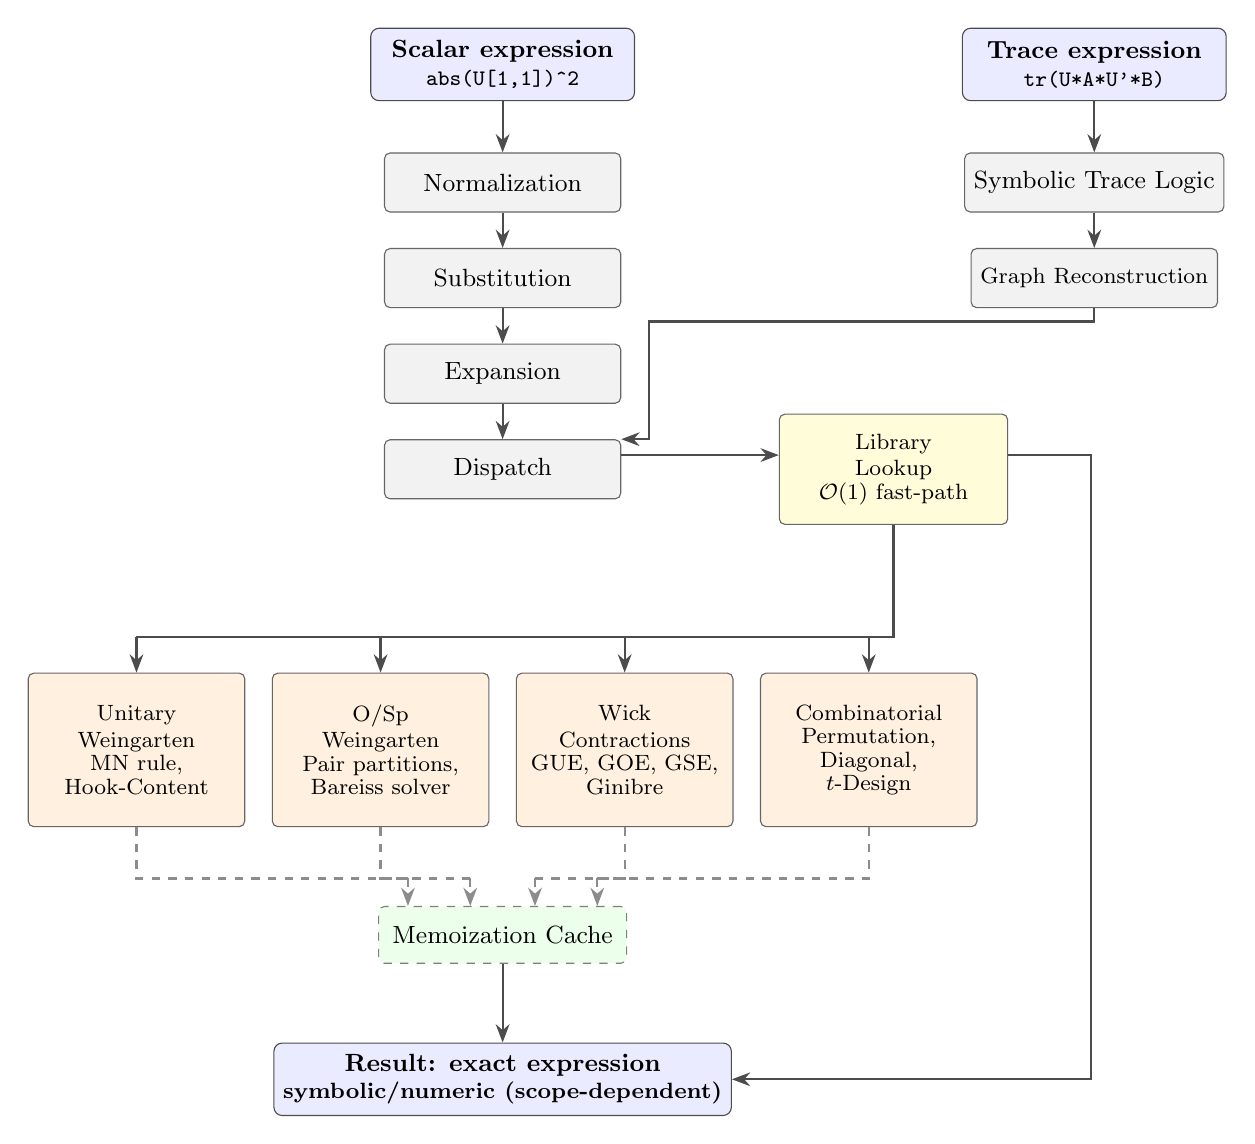
\begin{tikzpicture}[
    >=Stealth,
    node distance=0.65cm and 1.05cm,
    input/.style={
        rectangle, rounded corners=3pt, draw=black!70, fill=blue!8,
        minimum width=3.35cm, minimum height=0.92cm, align=center,
        font=\small\bfseries
    },
    pipeline/.style={
        rectangle, rounded corners=2pt, draw=black!60, fill=gray!10,
        minimum width=3.0cm, minimum height=0.75cm, align=center,
        font=\small
    },
    engine/.style={
        rectangle, rounded corners=2pt, draw=black!60, fill=orange!12,
        minimum width=2.75cm, minimum height=1.95cm, align=center,
        font=\footnotesize
    },
    cache/.style={
        rectangle, rounded corners=2pt, draw=black!50, fill=green!8,
        minimum width=3.15cm, minimum height=0.72cm, align=center,
        font=\small, dashed
    },
    output/.style={
        rectangle, rounded corners=3pt, draw=black!70, fill=blue!8,
        minimum width=4.75cm, minimum height=0.92cm, align=center,
        font=\small\bfseries
    },
    route/.style={thick, black!70},
    droute/.style={thick, black!45, dashed},
    arr/.style={route, ->},
    darr/.style={droute, ->},
]

% Top row: entry points
\node[input] (scalar) {Scalar expression\\[-1pt]\footnotesize\texttt{abs(U[1,1])\^{}2}};
\node[input, right=4.15cm of scalar] (trace) {Trace expression\\[-1pt]\footnotesize\texttt{tr(U*A*U'*B)}};

% Middle layers
\node[pipeline, below=0.65cm of scalar] (norm) {Normalization};
\node[pipeline, below=0.45cm of norm] (subs) {Substitution};
\node[pipeline, below=0.45cm of subs] (expand) {Expansion};
\node[pipeline, below=0.45cm of expand] (dispatch) {Dispatch};

\node[pipeline, below=0.65cm of trace] (trlogic) {Symbolic Trace Logic};
\node[pipeline, below=0.45cm of trlogic, font=\footnotesize] (graph) {Graph Reconstruction};

\node[engine, fill=yellow!15, minimum width=2.9cm, minimum height=1.4cm, right=2.0cm of dispatch]
    (library) {Library\\Lookup\\[-1pt]\footnotesize $\mathcal{O}(1)$ fast-path};

% Engine row
\coordinate (engine_row_anchor) at ($(dispatch.south)+(0,-2.2cm)$);
\node[engine, anchor=north] (wg_u) at ($(engine_row_anchor)+(-4.65cm,0)$)
    {Unitary\\Weingarten\\[-1pt]\footnotesize MN rule,\\[-1pt]\footnotesize Hook-Content};
\node[engine, anchor=north] (wg_o) at ($(engine_row_anchor)+(-1.55cm,0)$)
    {O/Sp\\Weingarten\\[-1pt]\footnotesize Pair partitions,\\[-1pt]\footnotesize Bareiss solver};
\node[engine, anchor=north] (wick) at ($(engine_row_anchor)+(1.55cm,0)$)
    {Wick\\Contractions\\[-1pt]\footnotesize GUE, GOE, GSE,\\[-1pt]\footnotesize Ginibre};
\node[engine, anchor=north] (comb) at ($(engine_row_anchor)+(4.65cm,0)$)
    {Combinatorial\\[-1pt]\footnotesize Permutation,\\[-1pt]\footnotesize Diagonal,\\[-1pt]\footnotesize $t$-Design};

% Cache + result rows
\node[cache, below=1.0cm of wg_o.south, xshift=1.55cm] (memo) {Memoization Cache};
\node[output, below=1.0cm of memo] (result) {Result: exact expression\\[-1pt]\footnotesize symbolic/numeric (scope-dependent)};

% Dedicated routing lanes
\coordinate (library_out) at ([yshift=0.18cm]library.east);
\coordinate (library_in) at ([yshift=0.18cm]library.west);
\coordinate (outer_lane_top) at ($(library_out)+(1.05cm,0)$);
\coordinate (outer_lane_bot) at ($(outer_lane_top |- result.east)$);
\coordinate (trace_over_lane) at ($(expand.north)+(0,0.28cm)$);
\coordinate (trace_drop) at ($(graph.south |- trace_over_lane)$);
\coordinate (trace_in) at (dispatch.north east);
\coordinate (trace_side) at ($(trace_in)+(0.35cm,0)$);
\coordinate (trace_turn) at (trace_side |- trace_over_lane);
\coordinate (wg_u_in) at ($(wg_u.north)+(0,0.45cm)$);
\coordinate (wg_o_in) at ($(wg_o.north)+(0,0.45cm)$);
\coordinate (wick_in) at ($(wick.north)+(0,0.45cm)$);
\coordinate (comb_in) at ($(comb.north)+(0,0.45cm)$);
\coordinate (fanout_hub) at (comb_in);
\coordinate (library_fallback_drop) at ($(library.south |- fanout_hub)$);

% Entry arrows
\draw[arr] (scalar) -- (norm);
\draw[arr] (trace) -- (trlogic);
\draw[arr] (trlogic) -- (graph);

% Scalar pipeline
\draw[arr] (norm) -- (subs);
\draw[arr] (subs) -- (expand);
\draw[arr] (expand) -- (dispatch);

% Trace merge to dispatch via an upper lane above the library lookup
\draw[arr] (graph.south) -- (trace_drop) -- (trace_turn) --
    (trace_side) -- (trace_in);

% Dispatch to library
\draw[arr] ([yshift=0.18cm]dispatch.east) -- (library_in);

% Library bypass to result via outer lane (avoids lower boxes)
\draw[arr] (library_out) -- (outer_lane_top) -- (outer_lane_bot) -- (result.east);

% Library fallback to engines through shared manifold and branch stubs above boxes
\draw[route] (wg_u_in) -- (fanout_hub);
\draw[route] (library.south) -- (library_fallback_drop) -- (fanout_hub);
\draw[arr] (wg_u_in) -- (wg_u.north);
\draw[arr] (wg_o_in) -- (wg_o.north);
\draw[arr] (wick_in) -- (wick.north);
\draw[arr] (comb_in) -- (comb.north);

% Engines to cache using separated cache targets
\coordinate (memo_in1) at ($(memo.north west)!0.12!(memo.north east)$);
\coordinate (memo_in2) at ($(memo.north west)!0.37!(memo.north east)$);
\coordinate (memo_in3) at ($(memo.north west)!0.63!(memo.north east)$);
\coordinate (memo_in4) at ($(memo.north west)!0.88!(memo.north east)$);
\coordinate (memo_bus) at ($(memo.north)+(0,0.35cm)$);
\coordinate (memo_bus1) at (memo_in1 |- memo_bus);
\coordinate (memo_bus2) at (memo_in2 |- memo_bus);
\coordinate (memo_bus3) at (memo_in3 |- memo_bus);
\coordinate (memo_bus4) at (memo_in4 |- memo_bus);

\draw[droute] (wg_u.south) -- (wg_u.south |- memo_bus) -- (memo_bus1);
\draw[droute] (wg_o.south) -- (wg_o.south |- memo_bus) -- (memo_bus2);
\draw[droute] (wick.south) -- (wick.south |- memo_bus) -- (memo_bus3);
\draw[droute] (comb.south) -- (comb.south |- memo_bus) -- (memo_bus4);
\draw[darr] (memo_bus1) -- (memo_in1);
\draw[darr] (memo_bus2) -- (memo_in2);
\draw[darr] (memo_bus3) -- (memo_in3);
\draw[darr] (memo_bus4) -- (memo_in4);

% Cache to result
\draw[arr] (memo.south) -- (result.north);

\end{tikzpicture}
\end{document}
